% !TEX encoding = UTF-8
% !TEX TS-program = pdflatex
% !TEX root = ../tesi.tex
% !TEX spellcheck = it-IT

%**************************************************************
\chapter{L'azienda e gli stage}
\label{cap:stage}
%**************************************************************

\intro{Dedico il presente capitolo al rapporto dell'azienda 
	con gli stage in collaborazione con l'Università degli 
	Studi di Padova. Nello specifico, presento: l'ambito, 
	le motivazioni, obiettivi aziendali e personali, e i 
	vincoli del mio progetto di stage.
}

%**************************************************************
\vspace{20pt}
L'azienda investe costantemente sui propri dipendenti per soddisfare i bisogni tecnologici del mercato con le giuste competenze. 
I dipendenti dell'azienda dedicano parte della propria giornata lavorativa in approfondimenti personali e attività di formazione. 

A supporto dell'attività di laboratorio, il team IT interno ha installato un ambiente virtuale. Disporre in azienda di un simile environment permette ai dipendenti di sperimentare con: tecnologie, integrazione di sistemi ed ecc. Inoltre, offre un'infrastruttura dedicata per i progetti di stage. I temi comuni di sperimentazione sono, invece, il  \textit{Cloud}, \textit{Machine Learning} e \textit{Analytics}. 

Di recente, l'Azienda ha concluso una partnership strategica con AWS (\textit{Amazon Web Services}). Quest'accordo, di collaborazione, permetterà a IKS di migrare verso il Cloud e beneficiare delle sue peculiarità, per esempio: elasticità, alta affidabilità, flessibilità nella gestione di infrastrutture ed ecc. 

Ogni anno, l'azienda partecipa a StageIT: un evento completamente dedicato agli studenti universitari dei Corsi di Laurea in Scienze e Ingegneria Informatica.
Infatti, StageIT permette  allo studente di mettersi in contatto diretto con le aziende e queste ultime di promuovere i propri progetti di stage. 
L'evento prevede, inoltre, un concorso per premiare il miglior progetto di stage svolto nell'edizione precedente. Il vincitore del concorso, scelto dagli studenti, ottiene come premio un buono d'acquisto del valore di 500 Euro.

\section{Il valore aggiunto di uno stagista}

IKS è un partecipante attivo a StageIT; annualmente l'azienda propone fino a 6 progetti di stage. Gli argomenti degli stage non sono verticali su un'unica 
tematica, ma coinvolgono temi come: 

\begin{itemize}
	\item Sviluppo di applicazioni basate su web, \gls{cloud}, mobile 
	      o migrazione su \gls{cloud}/mobile di applicazioni tradizionali;
	\item Progettazione di ambienti, metodologie e strumenti di 
	      sviluppo software.
\end{itemize}

Lo stagista è una risorsa importante per IKS; esso porta idee nuove e contribuisce a consolidare il valore aggiunto aziendale.
In principio, l'azienda impiega lo stagista su progetti di sperimentazione. Questi ultimi hanno come obiettivo l'analisi di fattibilità e lo studio dell'integrazione delle soluzioni nell'offerta commerciale dell'azienda. 

Per l'intera durata dello stage, lo stagista opera in un ambiente vero simile alla realtà aziendale. Il tutor esterno, oltre a guidare nel lavoro lo stagista in relazione a un PdL (Piano di Lavoro), osserva le attività dello stagista. 
Le osservazioni contribuiscono alla valutazione finale dell'attività di stage del tirocinante.

L'Azienda, con il contributo degli stagisti, allinea se stessa con i temi di ricerca universitari e con le tendenze tecnologiche del momento sul mercato internazionale.

\section{Alcuni temi di stage}
\subsection{AIOps e Machine Learning}
Il progetto di stage tratta l'integrazione del \textit{Machine Learning} con strumenti di Application Performance Monitoring. L'obiettivo dello 
stage è sperimentare integrando diverse soluzioni in questo ambito e studiarne il prodotto finale. Una conseguenza critica di questo progetto è lo sviluppo di un pensiero critico per affrontare le più difficili sfide del monitoraggio di applicazioni e infrastrutture. 

Il presente progetto si colloca nell'ambito del \textit{application and performance monitoring} che è un servizio offerto dall'azienda al supporto della governance IT. 


\subsection{DevOps Automazione}
L'automazione è fondamento di ogni realtà aziendale contemporanea. Infatti, il numero di macchine da gestire spesso non è piccolo. Per semplificare i compiti di gestione si devono utilizzare strumenti di configurazione e automazione. Queste tecnologie permettono di automatizzare tutte le operazioni 
manuali che un sistemista spesso compie durante le attività di manutenzione giornaliere. L'obiettivo di questo progetto è l'integrazione di alcuni strumenti che semplificano il \gls{patching} dei server e sperimentare con nuove tecnologie del settore.
Il presente progetto si colloca nell'ambito del \textit{system management}. 

\subsection{Sviluppo moduli evolutivi in ambito antifrode}
IKS ha grande esperienza in ambito della sicurezza informatica bancaria. Uno dei prodotti risultati di questa esperienza è SMASH. L'obiettivo dello stage è estendere il prodotto con qualche funzionalità di monitoraggio di azioni sospette. Oltre allo sviluppo di moduli evolutivi lo stagista ha la possibilità di apprendere delle competenze forti nell'ambito della 
sicurezza informatica. 
La presente proposta di stage è un progetto inter business unit dell'azienda. 
Esso si colloca nell'ambito dello sviluppo di prodotti software e della sicurezza informatica nel settore bancario.


\section{Il progetto proposto}
\subsection{Motivazioni}

E' sempre più comune, nelle realtà aziendali, l'approccio agile. Quest'approccio 
promuove la comunicazione e concentra l'attenzione di tutti i stakeholder sul valore 
finale di prodotto e/o strategia da raggiungere. 

Se gli sviluppatori hanno come obiettivo primario lo sviluppo di un prodotto software 
allora i professionisti dell'IT hanno come priorità la garanzia di servizio e manutenzione 
periodica del prodotto software realizzato. 

\begin{figure}[htbp]
	\begin{center}
		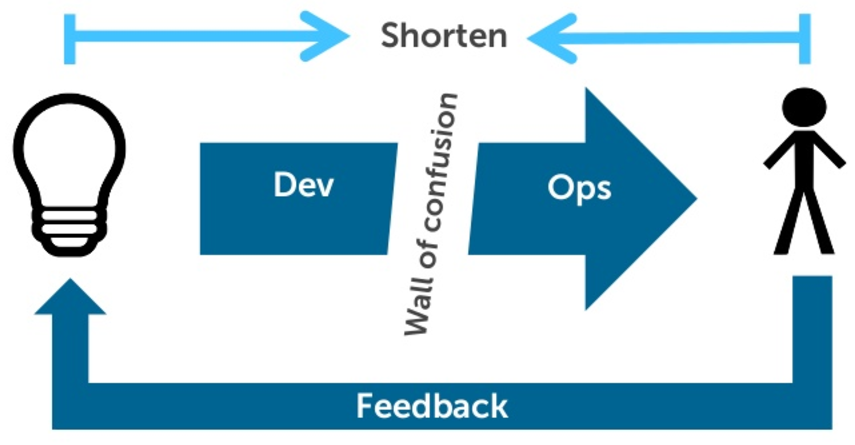
\includegraphics[height=4cm]{devops-wc}
		\caption{Sia gli sviluppatori che i professionisti IT sono portatori di valore: 
	    un feedback che coinvolge ambe le parti è essenziale. Immagine tratta 
		da: http://bit.ly/2rM9lBQ.}
	\end{center}
\end{figure}


Tra i due gruppi esiste un muro di incomprensione. La mancanza di comunicazione ed 
interazione rafforza questo fenomeno. Le problematiche, che avvengono dopo il rilascio del prodotto 
software, sono responsabilità dei professionisti IT. Di conseguenza, le loro attività 
sono orientate alla risoluzione dei problemi. Una simile organizzazione della distribuzione 
delle responsabilità è normale in contesti di realtà aziendali con rilasci sporadici.  

Un'azienda informatica, che deve affrontare un numero elevato di rilasci giornalieri, 
necessita di un approccio diverso. A questo scopo il movimento culturale, 
chiamato DevOps, è orientato all'unione degli sviluppatori e sistemisti. 
L'unione promuove un cambio di mentalità, creazione di nuove competenze e 
sviluppo di nuovi strumenti che diminuiscano la distanza tra le due realtà. 

Il DevOps ha conseguenze più profonde del semplice cambio culturale.  
Esso introduce un cambiamento interno orientato alla modifica del modello 
di qualità. I benefici di questo cambiamento sono i seguenti: maggiore 
innovazione, qualità di prodotto, processo e agilità nel cogliere i bisogni di mercato del momento.

Una tipica rappresentazione del ciclo di vita DevOps segue in figura. 

\begin{figure}[htbp]
	\begin{center}
		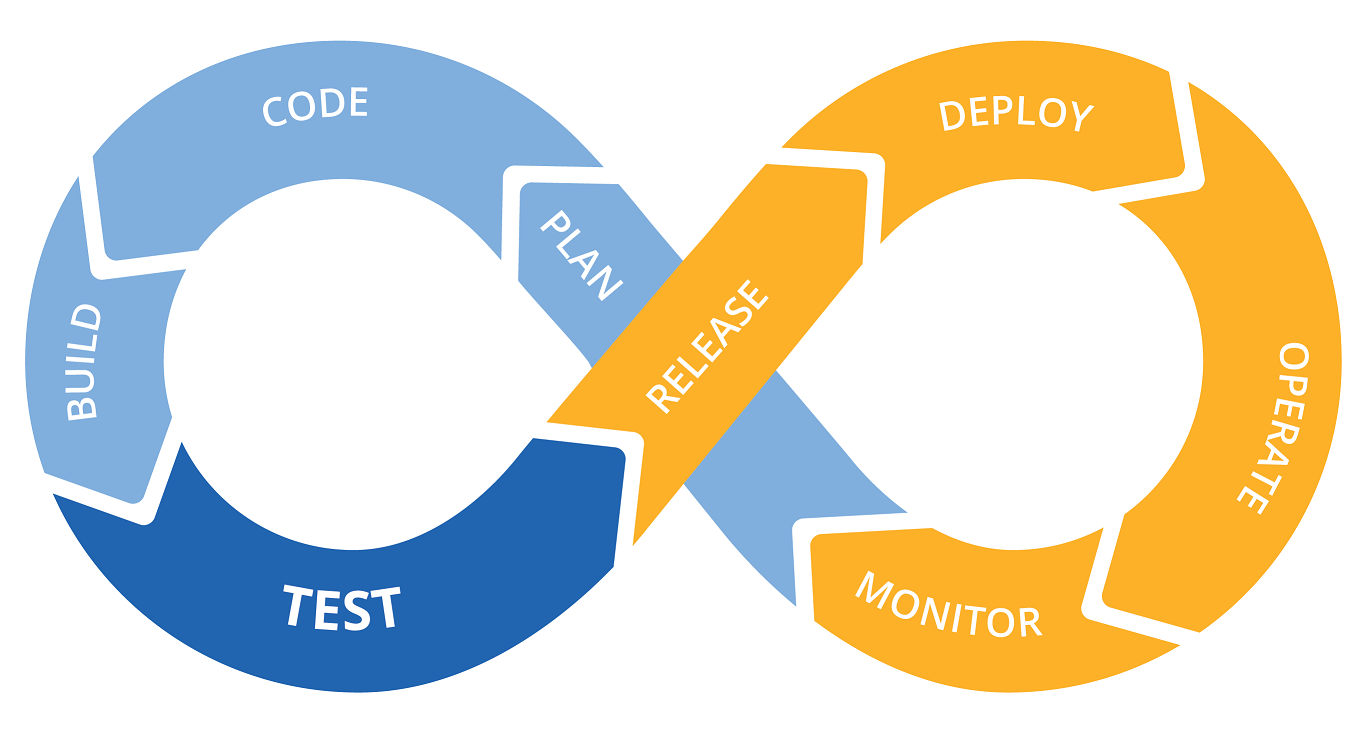
\includegraphics[height=4cm]{devops-pipeline}
		\caption{Il DevOps abilita l'automazione del processo di rilascio del software e i cambi dell'infrastruttura IT. Immagine tratta da: http://bit.ly/2rsw9nm.}
	\end{center}
\end{figure}

L'abilità di cambiare in modo agile è un grande beneficio per le aziende: il modo di lavorare diventa più flessibile e i dipendenti mostrano un maggior coinvolgimento nella quotidianità aziendale.    

Lato infrastrutturale, invece, la gestione diventa: disciplinata, sistematica e standardizzata. Con un approccio standardizzato e ben strumentalizzato è sempre più difficile individuare server nomadi. Può succedere che, in caso di operazioni sofisticate e mirate alla manutenzione, un server scompaia dall'orizzonte di visibilità. In assenza di opportuni strumenti è difficile individuare l'accaduto.   

Sebbene il DevOps possieda uno scopo più ampio, il \textit{continuous delivery} è un approccio che promuove l'automazione di tutti i processi coinvolti 
durante il rilascio di un prodotto software. Questo permette di abbreviare i tempi, aumentare il numero dei rilasci e migliorare la gestione del cambiamento.

Essere veloci nel \textit{delivery} di un prodotto software non è sufficiente. E' importante prevedere una \textit{pipeline} di \textit{deployment} che coinvolga ogni \textit{stage} del ciclo di \textit{operation}. Automatizzare il \textit{deployment} implica minor intervento manuale, minor numero di errori e conseguentemente maggiore formalità nelle attività complessive coinvolte. 

Un \textit{application container} permette di confezionare le applicazioni e dipendenze esterne in unità singole. Implementare il \textit{packaging} in questo modo le applicazioni facilita lo scambio di artefatti tra tutti i gruppi coinvolti nel ciclo di vita del prodotto software. Di conseguenza; sia il professionista IT che lo sviluppatore instaurano un protocollo di comunicazione e scambio di esperienze basato su qualcosa di concreto, stabile e funzionante.
Il classico detto "funziona sul mio computer" perde di significato.

Al momento la comunità open source offre molte tecnologie di containerizzazione. Quella più stabile e famosa nel comunità Linux è LXC (\textit{Linux Kernel Container}); questa tecnologia aggiunge il supporto a livello del kernel dei container applicativi per i sistemi operativi Linux. Docker, invece, è un'altra soluzione di containerizzazione. Le prime versioni di Docker interagivano con LXC; le versioni recenti di Docker hanno rimosso la dipendenza software verso LXC e ha implementato una soluzione di containerizzazione proprietaria. 

La containerizzazione è una tecnologia molto attraente. Visti i vantaggi tecnici, la containerizzazione porta a un livello superiore il modello concettuale rappresentante un'applicazione.  L'architettura dei prodotti software, dal punto di vista dei container, risulta essere più componibile. In un ambiente dinamico, caratterizzato dall'automazione, verifiche e \textit{deployment} automatici, le classiche architetture software non sono pensate per beneficiare di questa flessibilità. Lo stesso non vale per i  microservizi. 

I microservizi rappresentano uno stile architetturale in sintonia con la filosofia Unix: ogni microservizio implementa una sola funzionalità - basso accoppiamento.

\begin{figure}[htbp]
	\begin{center}
		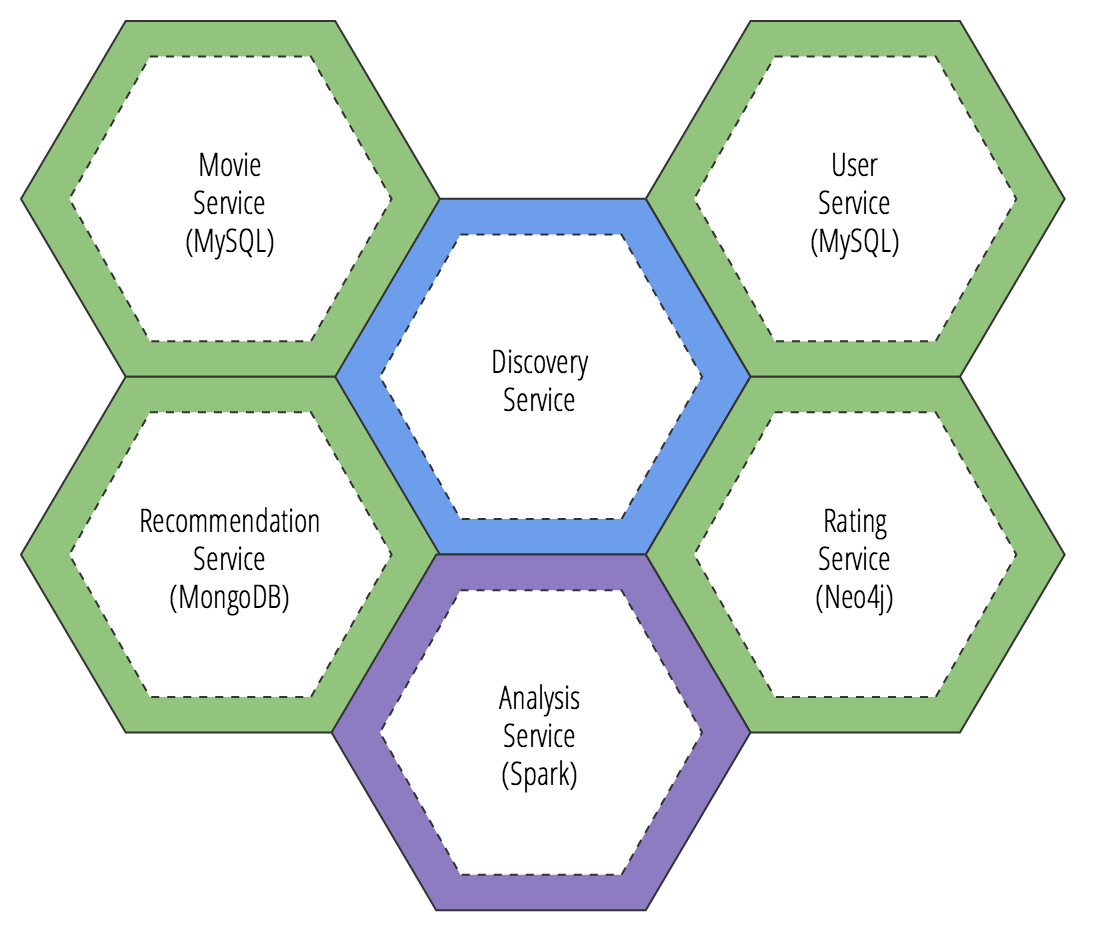
\includegraphics[height=5cm]{microservice-example}
		\caption{Esempio di un sistema a microservizi. Immagine tratta da: http://bit.ly/2qNXKxj.}
	\end{center}
\end{figure}

La figura presenta graficamente diversi microservizi. Ciascuno dei quali ha una responsabilità ben definita. Per garantire un basso accoppiamento tra i microservizi, il sistema deve utilizzare un servizio infrastrutturale e di supporto, chiamato \textit{Service Discovery}, utilizzato come un DNS (\textit{Domain Name System}). In questo modo, i microservizi continuano ad essere autonomi, mentre la gestione della comunicazione inter microservizio è separata dall'evoluzione dei singoli microservizi. 
In aggiunta, i microservizi beneficiano della \textit{space transparency}. Se un microservizio X, in esecuzione su una macchina A, migra per eseguire su una macchina B, allora un microservizio Y, che vuole comunicare con X, deve contattare il \textit{Service Discovery} per ottenere l'indirizzo di X. L'effetto ottenibile è un alto tasso di mobilità dei servizi.  

E' usuale incapsulare un microservizio in una capsula - il container software. Per la proprietà di isolamento: nello stesso ambiente possono coesistere due o più copie dello stesso microservizio, riducendo quasi a zero l'interferenza di un microservizio su un'altro. 
Con la scalabilità orizzontale i microservizi beneficiano dell'incremento in robustezza e alta affidabilità. Per implementare il \textit{routing} delle richieste verso i microservizi, i professionisti IT configurano un microservizio di \textit{load balancing} a livello applicativo del modello OSI (\textit{Open System Interconnection}).


\begin{figure}[htbp]
	\begin{center}
		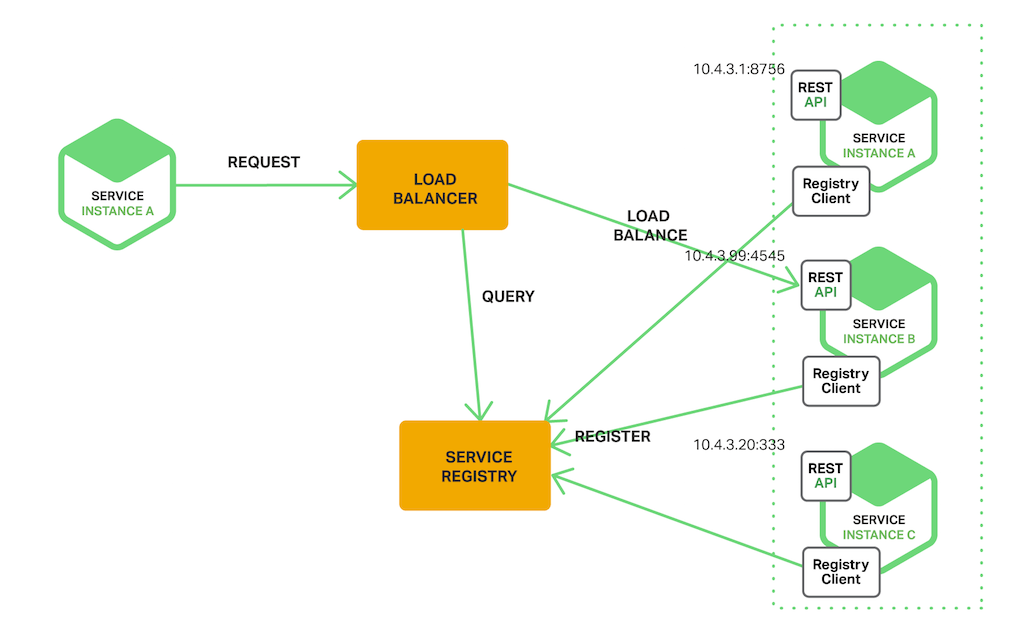
\includegraphics[height=6cm]{richardson-microservices}
		\caption{I microservizi permettono di scalare orizzontalmente per reggere ai più esigenti carichi di lavoro. Immagine tratta da: http://bit.ly/2qI50LR.}
	\end{center}
\end{figure}

I microservizi semplificano l'analisi, progettazione e implementazione dell'applicazione complessiva, scomponendo il prodotto complessivo in sotto applicazioni indipendenti; inoltre, i microservizi complicano l'applicazione a causa di: un elevato numero di componenti da gestire, difficoltà di versionare i microservizi in modo consistente e indipendente, politiche complesse di monitoraggio ed ecc. Per la tracciabilità delle richieste inter servizio è usuale utilizzare strumenti specializzati nel monitoraggio. Esempi di applicazioni, a questo scopo, sono: Appdynamics, Dynatrace, Instana ed ecc. 

I container e microservizi aprono nuove sfide sia per gli sviluppatori che per i sistemisti. E queste sfide caratterizzano il contratto di collaborazione tra i due gruppi. 


%%% ------------------------------------------------------------------------------

%%% -------------------------------------------------------------------------------

\subsection{Obiettivi aziendali}

Un team interno di IKS ha sviluppato una soluzione di Executive e Malware Dashboard
basata sullo stack applicativo: Elasticsearch, Logstash e Kibana.
 
La mia attività di stage ha avuto la containerizzazione della soluzione precedentemente implementata come obiettivo principale.

Di seguito presento gli obiettivi principali della mia attività di stage:

\begin{itemize}
	\item Containerizzare le componenti applicative, costituenti la soluzione implementata dal team interno di IKS; 
	\item Garantire la non regressione al livello funzionale della soluzione;
	\item Predisporre un ambiente containerizzato con e senza orchestratore di container.
\end{itemize} 

In conclusione, la containerizzazione garantisce che la soluzione di executive e malware dashboard sia portabile su ambienti diversi, dal portatile del sviluppatore al Cloud.  

\subsection{Obiettivi personali}
Come attività preliminare alla ricerca di un progetto di stage per la Laurea ho 
attuato uno studio individuale di mercato. Lo scopo era capire: tendenze 
tecnologiche, architetturali e metodologiche. Se da un lato le mie ricerche 
hanno cercato di cogliere le novità del momento, dall'altro a livello personale 
queste erano mirate alla ricerca di un contesto in cui potermi applicare e maturare. 

Con il presente progetto gli obiettivi personali erano:

\begin{itemize}
	\item Apprendere conoscenze e competenze in ambito di:
		\begin{itemize}
			\item Virtualizzazione basata sulla tecnologia a container; 
			\item Sistemi distribuiti;
			\item Amministrazione di sistema Linux;
	    \end{itemize}
	\item Acquisire esperienza pratica nella gestione delle reti di calcolatori in ambito dei sistemi, nello specifico le reti definite in modo programmatico per le tecnologie orientate alla containerizzazione; 
	\item Acquisire esperienza nell'analisi, progettazione e implementazione di sistemi orientati ai microservizi;
	\item Famigliarizzare con la piattaforma Kubernetes e i principi del \gls{cloud}.
\end{itemize} 

\section{Piano di lavoro}
\label{sec:piano-di-lavoro}
L'azienda ha pianificato un piano di lavoro (PdL) per un totale di 300 ore complessive. 
Ho consegnato il documento del PdL all'Ufficio degli Stage presso l'Ateneo dell'Università di Padova; una seconda copia del PdL ho consegnato al tutor interno; l'ultima copia, invece, 
controfirmata dall'ufficio stage dell'Università ho consegnato all'azienda.

Descrivo brevemente di seguito il contenuto del PdL inerente all'insieme delle attività svolte:
\begin{itemize}
\item Fase 1 - Formazione  (56 ore)
	\begin{itemize}
		\item Docker: la tecnologia per la containerizzazione;
		\item Kubernetes: la tecnologia per l'orchestrazione;
		\item Elasticsearch, Logstash e Kibana (ELK): lo stack applicativo;
		\item Verifiche delle competenze acquisite;
	\end{itemize}
\item Fase 2 - Analisi e progettazione  (56 ore)
	\begin{itemize}
		\item Analisi delle funzionalità della soluzione non containerizzata di dashboard;
		\item Analisi delle modalità di containerizzazione delle componenti;
		\item Analisi delle modalità di \textit{deployment};
		\item Progettazione delle modalità di verifica della non regressione;
		\item Progettazione architetturale della soluzione; 
		\item Progettazione della modalità di \textit{deployment};
		\item Documentazione;
	\end{itemize}
\item Fase 3 - Implementazione  (188 ore)	
	\begin{itemize}
		\item Installazione e configurazione dell'orchestratore;
		\item Implementazione della soluzione in un contesto con e senza orchestratore;
		\item Verifica di non regressione;
		\item Documentazione.
	\end{itemize}
\end{itemize}

\section{Vincoli}
\subsection{Vincoli temporali}
Lo stage ha avuto una durata di 8 settimane, per un complessivo di 310 ore di lavoro. Ho lavorato a tempo pieno con il seguente orario: 9.00-18.00. Con la pausa pranzo di 1 ora dalle 12.30 alle 13.30. Come pianificato nel PdL,  ho seguito le attività in ordine seguendo le fasi della pianificazione. Qualche volta ho alterato l'ordine delle attività per adattare le esigenze e ridurre gli effetti del cambio di contesto.  Infatti, ogni fase ha coinvolto attività mirate al raggiungimento di specifici obiettivi. Per maggior dettaglio sul contenuto del PdL riferire la \hyperref[sec:piano-di-lavoro]{sezione Piano di Lavoro}.

\subsection{Vincoli tecnologici}

Fin dal primo giorno di lavoro l'azienda mi ha fornito un portatile dedicato per l'itero periodo di stage. Inoltre, mi è stato vietato di collegare alla rete aziendale qualsiasi dispositivo personale. Inoltre, il portatile di lavoro non poteva essere portato a casa.
Per comunicare internamente sono stati utilizzati strumenti di messaggistica istantanea, come Skype, per comunicazioni informali e la posta elettronica.

Oltre a questo vincolo, a livello tecnologico sono state fissate le seguenti tecnologie:

\begin{itemize}
	\item CentOS7: il sistema operativo installato sulle macchine di laboratorio. CentOS7 è la versione open source di RHEL7 (Red Hat Enterprise Linux versione 7);
	\item Docker: lo strumento che permette in modo estremamente facile la creazione, il \textit{deployment} e l'esecuzione di applicazioni utilizzando la tecnologia a container. In questo modo l'utente focalizza l'attenzione su questioni diverse dall'installazione e configurazione dell'applicazione. 
	L'architettura di Docker segue in figura. 
	
	\begin{figure}[htbp]
		\begin{center}
			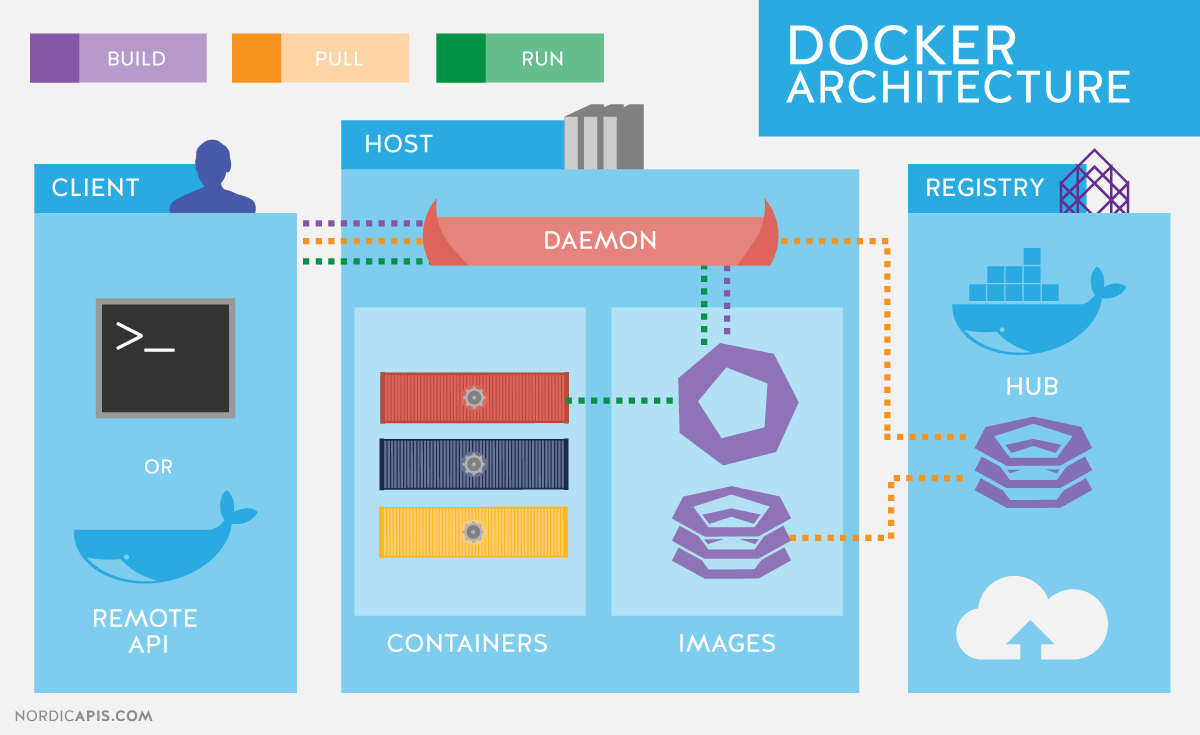
\includegraphics[height=6cm]{docker-architecture}
			\caption{Le parti costituenti la piattaforma Docker sono: il demone, il client e il registry Docker. Immagine tratta da: http://bit.ly/2rmkt7g.}
		\end{center}
	\end{figure}
	
	Le componenti architetturali costituenti la piattaforma Docker sono il:
	demone, client e registry. L'architettura di alto livello è 
	un architettura client/server. Il server di Docker è il demone che ha la responsabilità di gestione dei container sulla macchina locale. Mentre il client si interfaccia tramite un'interfaccia REST al demone e permette di interagire in modo agile con i container, creare reti virtuali, gestire i dati che devono essere condivisi tra i container e il file system locale della macchina. Infine, il registry di Docker è una repository che può essere pubblica o privata e ha la responsabilità di abilitare la condivisione di immagini utili alla creazione dei container. Come modello mentale, in relazione con il paradigma ad oggetti, è possibile paragonare le immagini Docker a classi che devono essere istanziate per la creazione di oggetti, ovvero container. 
	
	Per favorire il libero scambio di immagini Docker, l'azienda Docker Inc ha 
	messo a disposizione degli utenti un hub: spazio web per la condivisione delle immagini Docker. Nella modalità privata di una repository, Docker Inc rende disponibile 
	il servizio di \textit{scanning} delle vulnerabilità delle immagini. 
	
	Quando l'utente esegue il comando run tramite la CLI di Docker, il demone controlla che l'immagine da istanziare, per la creazione del container, sia presente sul \textit{file system} locale. In caso affermativo, il demone Docker crea e mette in esecuzione il container, altrimenti esso scarica prima l'immagine dal registry e al termine, di questa attività, istanzia il container;
	\item Kubernetes: è un sistema open source per automatizzare il \textit{deployment}, la scalabilità e gestione di applicazioni containerizzate. La tecnologia è il 
	risultato di 15 anni di esperienza in Google con la tecnologia a container. 
	Kubernetes garantisce la portabilità delle applicazioni e l'indipendenza dall'ambiente fisico di esecuzione.
	
	Kubernetes è un sistema distribuito per l'orchestrazione di container applicativi. Il modello architetturale dell'orchestratore è master/slave.
	
	\begin{figure}[htbp]
		\begin{center}
			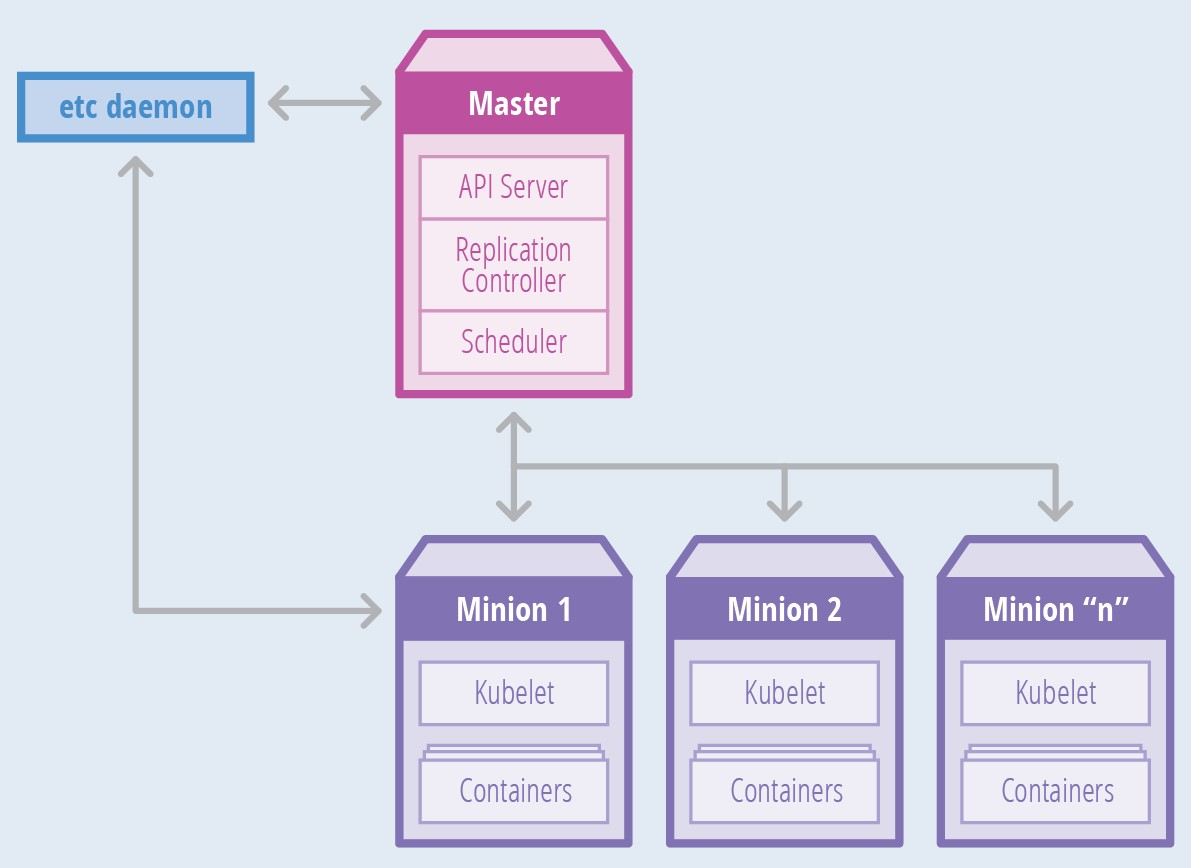
\includegraphics[height=6cm]{kube-architecture}
			\caption{Le componenti architetturali di Kubernetes sono: API server, Scheduler, Replication Contoller, Kubelet, Kube proxy, Database Etcd. Immagine tratta da: http://bit.ly/2s4eKUR.}
		\end{center}
	\end{figure}
	
	Il master è un pannello di controllo del sistema K8s (Kubernetes). Lui gestisce il \textit{workload} dei container. Inoltre, esegue le componenti critiche del sistema: il database chiave valore ad alta consistenza \textbf{etcd}, il gestore delle repliche per la scalabilità orizzontale - \textbf{replication controller} e lo \textbf{scheduler}.  
	
	La componente slave esegue il carico di lavoro. Essa comunica solo con il master e salva le informazioni di servizio, tramite il API server, nel database etcd. 
	
	Ogni componente master e slave eseguono un agente locale chiamato Kubelet. L'agente collega le varie componenti e interagisce con il demone Docker. 
	
	Infine, il Kube Proxy è la componente che gestisce il traffico di rete dell'intera infrastruttura. 
	
    Kubernetes, essendo un sistema fin dall'inizio pensato per essere componibile 
    si può integrare bene con soluzioni di terzi parti, come per esempio: diverse soluzioni per lo storage, diversi plugin per la rete ed ecc;
	
	\item Elasticsearch, Logstash e Kibana: Le tre componenti sono comunemente conosciute con l'acronimo ELK.  Esse vengono utilizzate insieme come una soluzione open source in progetti che hanno forti esigenze di ricerca e analisi di dati. Elasctisearch è il cuore dello stack applicativo. Esso è un database NoSQL e distribuito implementato in Java. Orientato all'immagazzinamento di dati non strutturati, Elasticsearch permette di effettuare ricerche complesse impiegando millisecondi contro i secondi necessari utilizzando un classico DB SQL.
	
	\begin{figure}[htbp]
		\begin{center}
			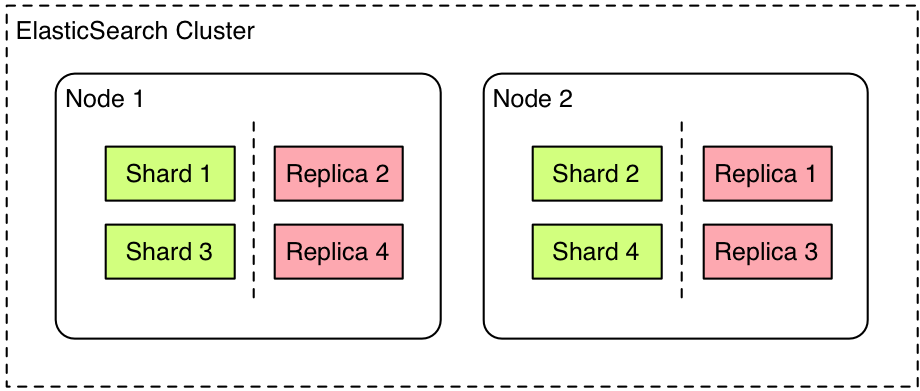
\includegraphics[height=4cm]{es-cluster}
			\caption{Vista di alto livello del meccanismo di partizione dei dati immagazzinati in Elasticsearch. Immagine tratta da: http://bit.ly/2r0HTQL.}
		\end{center}
	\end{figure}

	Il meccanismo di gestione dei dati di Elasticsearch è complicato. In figura è rappresentato un cluster di due nodi. Elasticsearch permette di organizzare l'insieme complessivo di dati in sottoinsiemi (\textit{shard}) e aggiungere un numero y di copie (\textit{replica}) per ogni sottoinsieme primario. Una simile organizzazione permette di garantire un'alta affidabilità di dati 
	a livello applicativo. Inoltre, in funzione ai casi d'uso Elasticsearch è altamente personalizzabile.
	Per incrementare le performance di lettura, l'utente incrementa il numero delle repliche. Per incrementare le performance di scrittura, l'utente diminuisce il numero di sottoinsiemi primari dei dati. 	
	Kibana, invece, è la componente dello stack che offre la funzionalità di visualizzazione dei dati presenti in Elasticsearch. Una peculiare caratteristica di Kibana è l'interfaccia di creazione dei cruscotti. Kibana sfrutta l'integrazione nativa con Elasticsearch per esprimere ricerche molto complesse e renderizzarle a video tramite effetti grafici accattivanti. Infine, Logstash è la componente di estrazione, trasformazione e caricamento dei dati dalla sorgente in Elasticsearch. Con Logstash risulta semplice filtrare l'informazione utile per l'analisi dei dati ed eliminare il rumore di fondo. La comunità open source di Logstash ha sviluppato un insieme molto ricco di strumenti che estendono il suo insieme di funzionalità. Per esempio, tramite uno plugin esterno è possibile programmare Logstash a interagire con le API (Application Program Interface) del social network Twitter, per cercare, scaricare e filtrare l'informazione che soddisfa uno specifico criterio di ricerca. 
	Dal punto di vista architetturale la soluzione ELK è flessibile e permette di scalare facilmente in orizzontale, proporzionalmente al carico di lavoro. 
	A seguire allego una rappresentazione grafica delle dipendenze inter componenti a livello architetturale. Infatti, Kibana legge da Elasticsearch (ES) mentre Logstash scrive in ES.
	
	\begin{figure}[htbp]
		\begin{center}
			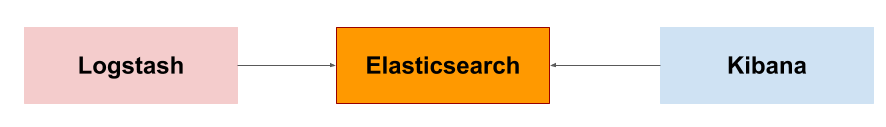
\includegraphics[height=1.5cm]{dipendenze-es}
			\caption{Vista di alto livello del legame sussistente inter componente. Il verso della freccia nell'immagine indica una dipendenza.}
		\end{center}
	\end{figure}
	
	  	
\end{itemize}

Inizialmente sono state fissate anche le rispettive versioni delle componenti sopra citate. Tuttavia, nel corso dello stage ho realizzato che questo può bloccare l'evoluzione dell'infrastruttura e comportare qualche problema in futuro. A questo scopo ho predisposto un ambiente tollerante agli aggiornamenti. Durante la personalizzazione dell'ambiente mi sono ispirato al principio  \textit{self driven infrastructure} di CoreOS. 
In questo modo gli aggiornamenti delle componenti possono essere effettuati in modo completamente trasparente.

Infine, come vincolo per le immagini dei container Docker mi hanno imposto di utilizzare solo le immagini ufficiali provenienti dal hub di Docker. Questo vincolo è dovuto alla presenza di vulnerabilità di sicurezza nelle immagini di terzi parti.